\documentclass[12pt]{article}
\usepackage[usenames]{color} %used for font color
\usepackage{amssymb} %maths
\usepackage{amsmath} %maths
\usepackage[utf8]{inputenc} %useful to type directly diacritic characters
\usepackage[T1]{fontenc}
\usepackage{polski}
\usepackage{pdfpages}

% \usepackage{listings}
\usepackage[theme=default-plain]{jlcode} % https://github.com/wg030/jlcode
\usepackage{graphicx}  %grafika

%\usepackage{subcaption} %dwa rysunki obok siebie
%\graphicspath{ {./rysunki/} } %skąd ma pobierać grafikę
%\usepackage{svg} % for graphics in svg, with the first compilation enable: "-shell-escape" to use tools to convert svg
%\usepackage{csvsimple} % to insert csv files 

\usepackage[a4paper, left=3cm, right=3cm, top=1cm, bottom=2cm]{geometry}



\title{Porównanie różnych metod numerycznego rozwiązywania liniowego układu równań różniczkowych}
\author{Bartosz Zbik}
\date{2024-03-02} %format jest dowolny(może być nawet miesiąc słownie

\begin{document}
\maketitle %tworzy tytuł dokumentu

Numerycznie rozwiąż:
\begin{equation}
\begin{cases}
\dot x = 1023 x + 2023 y \\
\dot y = -1024 x - 2024 y \\
x(0) = 1,\quad y(0) = 0
\end{cases}
\end{equation}

Rozwiazanie chcemy dostać na przedziale $t \in [0, 0.125]$. Użyj trzech metod:
\begin{itemize}
\item Jawnej metody Eulera (z różnymi krokami czasowymi $\Delta t = 1/256, 1/512, 1/2048$)
\item Runge-Kutta (z różnymi krokami czasowymi $\Delta t = 1/256, 1/512, 1/2048$)
\item Niejawna metoda Eulera  ($h = 1/256, 1/512, 1/2048$)
\end{itemize}

\textbf{Niejawna metoda Eulera:} Dany jest problem
\begin{equation}
\begin{cases}
\dot y = f(t, y) \\
y(0) = y_0
\end{cases}
\end{equation}
Robimy dyskretyzację i pochodną liczymy "w punkcie docelowym", a nie w punkcie w który jesteśmy
\begin{equation}
y_{n+1} = y_n + h f(t_{n+1}, y_{n+1})
\end{equation}
Generalnie to jest trudniejsze, ale dla r. liniowego dacie radę to odwikłać.


\section{Kod}
%\jlinputlisting{solution.jl}



\section{Wizualizacja wyników}
%\clearpage

\begin{figure}
\centering
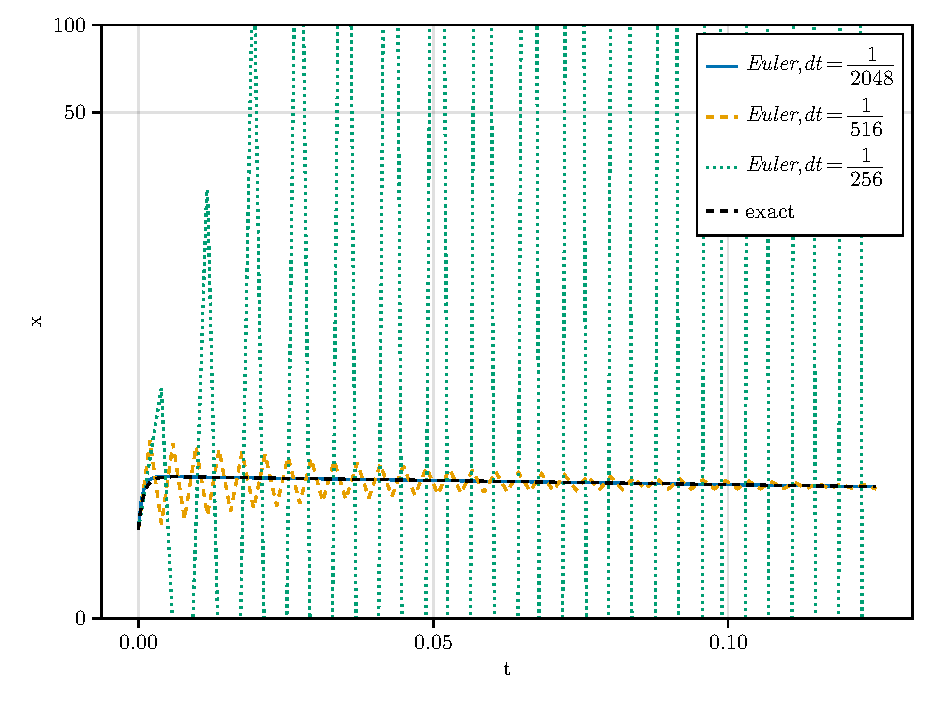
\includegraphics[width=\textwidth]{euler-methods}
\caption{Jawna metoda Eulera z różnym krokiem czasowym.}
\end{figure}

\begin{figure}
\centering
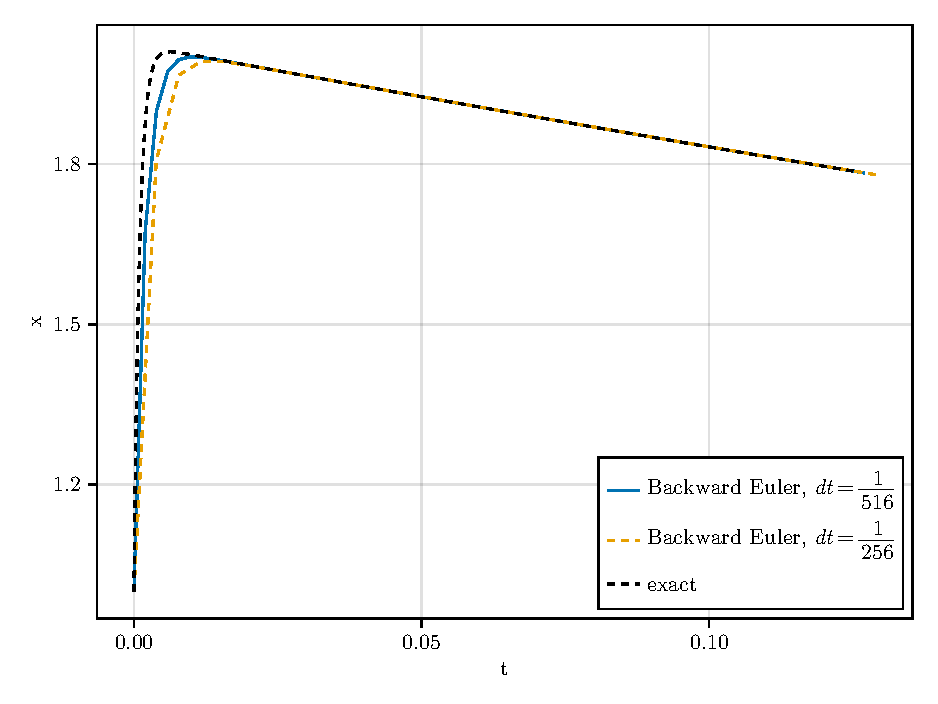
\includegraphics[width=\textwidth]{BE-methods}
\caption{Niejawna metoda Eulera z różnym krokiem czasowym. Tutaj konieczne jest zainwestowanie pewnej dodatkowej wiedzy o równaniu (trzeba odwrócić relację między $x_{n+1}$, a $x_n$.}
\end{figure}

\begin{figure}
\centering
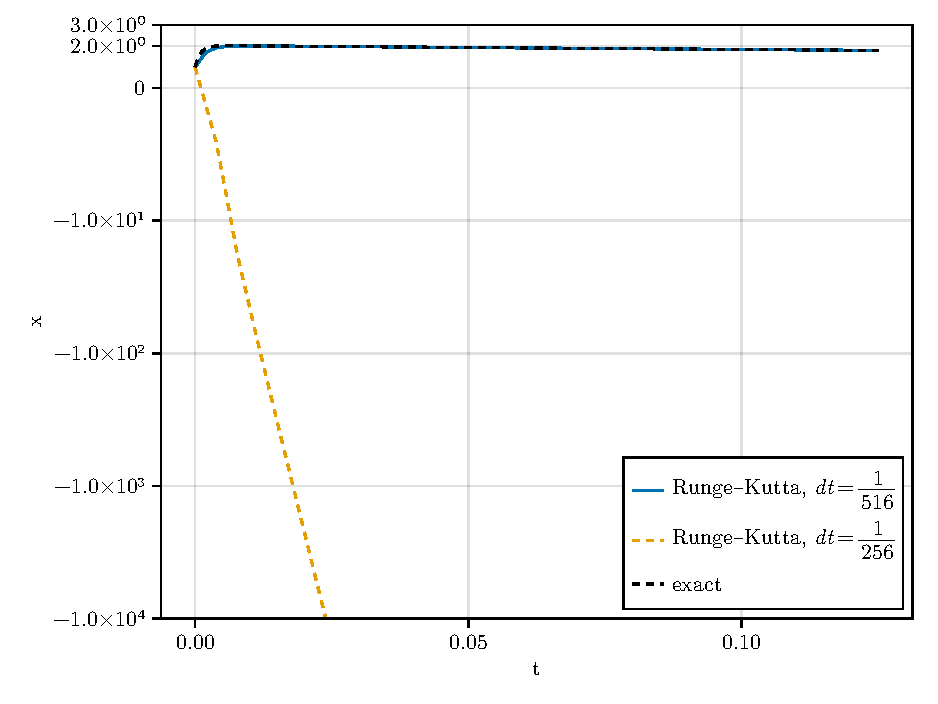
\includegraphics[width=\textwidth]{RK-methods}
\caption{Czterokrokowa metoda Rungego-Kutty ze stałym krokiem czasowym (nieadaptowalna)}
\end{figure}

\begin{figure}
\centering
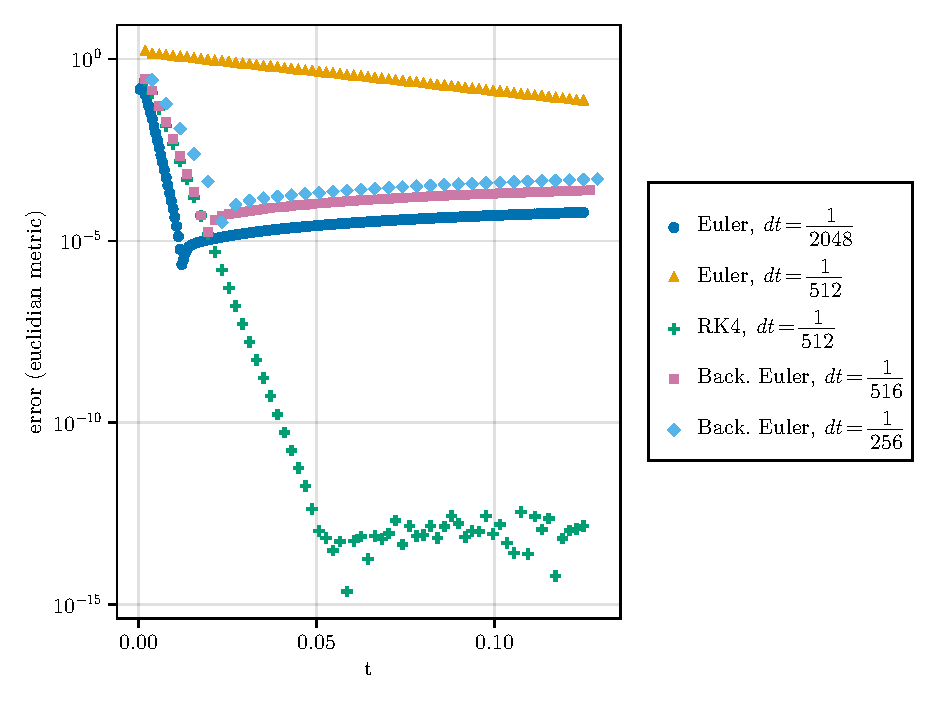
\includegraphics[width=\textwidth]{method-errors}
\caption{Porównanie błędów numerycznych jakimi obarczone były rozwiązania poszczególnymi metodami.}
\end{figure}



\end{document}